\section{Smíšené strategie}
\subsection{Definice konečné hry}
Nechť $G = (N, (S_i)_{i=1}^n, (u_i)_{i=1}^n)$ je strategická hra. Řekněme, že $G$ je konečná, jestliže pro každé 
$i \in N$ je $S_i$ konečná množina.

\subsection{Definice smíšeného rozšíření}
Nechť $G = (N, (S_i)_{i=1}^n, (u_i)_{i=1}^n)$ je konečná strategická hra $N = \bc{1, \dots, n}$ a pro každé $i \in N$ je
$S_i = \bc{\sigma_1^i, \dots, \sigma_{m_i}^i}$. Smíšené rozšíření $G$ je strategická hra 
$\overline{G} = (N, (\Delta S_i)_{i=1}^n, (U_i)_{i=1}^n)$, kde pro každé $i \in N$ je
\begin{itemize}
    \item $\Delta S_i = \bc{x \in \R_+^{m_i} \middle| \sum_{j=1}^{m_i}x_j = 1}$ množina všech smíšených strategií 
    (loterií) nad $S_i$,
    \item $U_i : \Delta S_1 \times \dots \times S_n \rightarrow \R$ je dána předpisem
    \[
        U_i (p^1, \dots, p^n) = \sum_{j_1 = 1}^{m_1} \dots \sum_{j_n=1}^{m_n} u_i(\sigma_{j_1}^1, \dots, \sigma_{j_n}^n)
        p_{j_1}^1 \dots p_{j_n}^n.
    \]
\end{itemize}
Pozorování.
\begin{itemize}
    \item Prvek $\sigma_k^i$ ztotožňujeme s prvkem $\R_+^{m_i}$, který má na $k$-té posici jedničku a všude jinde nuly.
    \item Prvky z $\Delta S_i$, které mají na jedné posici jedničku a na ostatních nulu, nazýváme 
    \textbf{čisté strategie}.
\end{itemize}

\subsection{Příklad Panna nebo orel}

\begin{multicols}{2}
    Hra je daná tabulkou:
    \[
    \begin{array}{|c| |c|c|}
        \hline
        & P & O \\ \hline \hline
        P & \phantom{-}10 & -10 \\ \hline
        O & -10 & \phantom{-}10 \\ \hline
    \end{array}
    \]

    $S_1 = S_2 = \bc{P, O}$

    $u_1 (P, P) = - u_2(P,P) = 10$\\
    $u_1 (P, O) = - u_2(P,O) = -10$\\
    $u_1 (O, P) = - u_2(O,P) = 10$\\
    $u_1 (O, O) = - u_2(O,O) = -10$\\
    $\sigma_1 = \tau_1 = P,\, \sigma_2 = \tau_2 = O$

\end{multicols}
$\Delta S_1 = \Delta S_2 = \bc{x \in \R_+^2 \middle| x_1 + x_2 = 1}$

\[  
    U_1(p,q) = \sum_{i=1}^{2} \sum_{j=1}^{2} u_1 (\sigma_i, \tau_i)p_i q_j = 
    10p_1q_1 + (-10)p_2q_1 + (-10)p_2q_2 + 10p_2q_2
\]
Zřejmě $U_2(p,q) = -U_1(p,q)$. $\implies \overline{G} = (\Delta S_1, \Delta S_2, U)$, kde $U = U_1$, tedy jedná se o hru
dvou hráčů s nulovým součtem.

Najděme optimální strategie.

Položme $p_1 = x,\, q_1 = y$. Pak $x, y \in [0,1]$, $p_2 = 1-x, \, q_2 = 1-y$.
\[
    \widetilde{U}(x,y) = 10xy - 10x(1-y) - 10(1-x)y + 10(1-x)(1-y) = 40xy -20x - 20y + 10 = 10(4xy - 2x - 2y + 1)
\]
Místo $\overline{G}$ uvažme hru $\Gamma = \left([0,1], [0,1], \widetilde{U}\right)$.

Hledejme Nashovo equilibrium hry $\Gamma$.

Použijeme \hyperref[cenaHry]{definici ceny hry}:
\begin{align*}
    \underline{v} = \max_{x \in [0,1]} \min_{y \in [0,1]} \widetilde{U}(x,y) \\
    \overline{v}  = \min_{y \in [0,1]} \max_{x \in [0,1]} \widetilde{U}(x,y)
\end{align*}
Spočtěme 
\begin{align*}
    \min_{y \in [0,1]} \widetilde{U}(x,y) &= \min_{y \in [0,1]} 10(4xy - 2x - 2y + 1) \\
    &= 10 \min_{y \in [0,1]} (4x-2)y -2x + 1=
    \begin{cases}
        10(-2x + 1) & x \geq \frac{1}{2} \\
        10(2x - 1)  & x < \frac{1}{2}
    \end{cases}
\end{align*}
\begin{multicols}{2}
    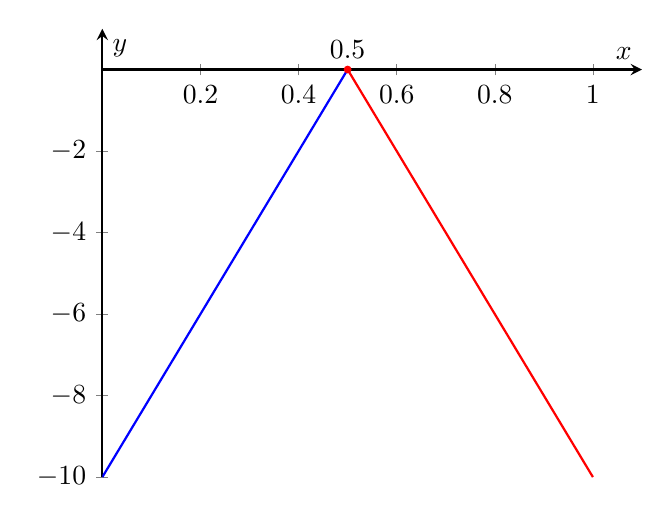
\begin{tikzpicture}
        \begin{axis}[
            axis lines=middle, 
            xmin=0, xmax=1.1,
            ymin=-10, ymax=1,
            xlabel={$x$}, ylabel={$y$},
            samples=200,
            domain=0:1,
            thick
        ]
            \addplot[blue, domain=0:0.5] {10 * (2 * x - 1)};
            \addplot[red, domain=0.5:1] {10 * (-2 * x + 1)};

            \node[fill=red, circle, inner sep=1pt] at (0.5, 0) {};
            \node at (0.5, 0.5) {0.5};
        \end{axis}
    \end{tikzpicture}

    $\implies \underline{v} = 0$
\end{multicols}
\begin{align*}
    \max_{x \in [0,1]} \widetilde{U}(x,y) &= \max_{x \in [0,1]} 10(4xy - 2x - 2y + 1) \\
    &= 10 \max_{x \in [0,1]} (4y-2)x -2y + 1 =
    \begin{cases}
        10(2y - 1) & y \geq \frac{1}{2} \\
        10(-2y + 1)  & y < \frac{1}{2}
    \end{cases}
\end{align*}
\begin{multicols}{2}
    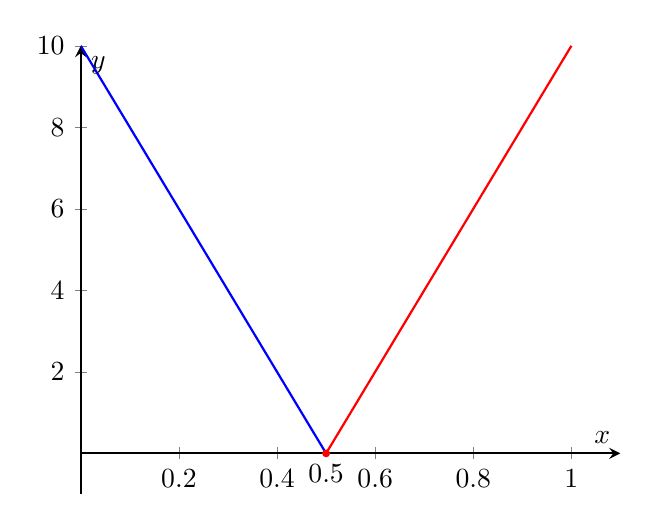
\begin{tikzpicture}
        \begin{axis}[
            axis lines=middle, 
            xmin=0, xmax=1.1,
            ymin=-1, ymax=10,
            xlabel={$x$}, ylabel={$y$},
            samples=200,
            domain=0:1,
            thick
        ]
            \addplot[blue, domain=0:0.5] {10 * (-2 * x + 1)};
            \addplot[red, domain=0.5:1] {10 * (2 * x - 1)};

            \node[fill=red, circle, inner sep=1pt] at (0.5, 0) {};
            \node at (0.5, -0.5) {0.5};
        \end{axis}
    \end{tikzpicture}

    $\implies \overline{v} = 0$
\end{multicols}
Tedy $\underline{v} = \overline{v} = v = 0$. Z grafu vyčteme, že optimální strategie 1. hráče je $x=\frac{1}{2}$ a 
optimální strategie 2. hráče je $y = \frac{1}{2}$ pro hru $\Gamma$.\\
\hyperref[nash]{Nashovo equilibrium} hry $\overline{G} = 
\left(\frac{1}{2}\begin{bmatrix}1 \\ 1\end{bmatrix}, \frac{1}{2}\begin{bmatrix}1 \\ 1\end{bmatrix}\right)$.

\subsection{Nashova věta}
Smíšené rozšíření konečné strategické hry má nejméně jedno \hyperref[nash]{Nashovo equilibrium}.

Důkaz vynecháme.